\documentclass[runningheads,a4paper]{article}
\usepackage[utf8]{inputenc}
\setcounter{tocdepth}{3}
\usepackage[english]{babel} 
\usepackage{graphicx}
\usepackage{grffile}
\usepackage{float}
\usepackage{multicol}
\usepackage{url}
\usepackage{titling}
\usepackage[hidelinks]{hyperref}
\setcounter{secnumdepth}{5}
%Margins
\usepackage[
margin=2cm,
includefoot
]{geometry}
\graphicspath{{img/}}
%Headers and Footers
\usepackage{fancyhdr}
\pagestyle{fancy}
\fancyhead{}
\fancyfoot{}
\fancyfoot[R]{\thepage}
\renewcommand{\headrulewidth}{0pt}
\renewcommand{\footrulewidth}{0pt}
\setlength\parindent{24pt}
\begin{document}
%Title Page
\begin{titlepage}
\begin{center}

\includegraphics[width=10cm]{UP.jpg}  \\
[1cm]
\line(1,0){300} \\
[0.3cm]
\textsc{\Large
NavUP \\
Architectural Requirements Specifications and Design \\
\hfill \break 01 March 2017
%University of Pretoria
}\\
[0.1cm]
\line(1,0){300} \\
[0.7cm]
\textsc{\Large
Team MatLab
} \\
\end{center}
\begin{center}
\begin{multicols}{2}
\textsc{\large\\
Frederick Ehlers\\ 
u11061112\\ 
}
\textsc{\large\\
Vignesh Iyer\\
u15031625\\ 
}
\textsc{\large\\
Stephanie Groutsch\\
u14293324\\ 
}
\textsc{\large\\
Neo Thokoa\\
u14163285\\
}
\columnbreak
\textsc{\large\\
Nokuthula Manana\\
u12064115\\
}
\textsc{\large\\
Jacobus Marais\\
u15188397\\
}
\textsc{\large\\
Heinrich Burgers\\
u15059538\\
}
\end{multicols}
\textsc{	\\ \href{https://github.com/FredJEhlers/Matlab}{GitHub}
\url{https://github.com/FredJEhlers/Matlab}}
\end{center}
\end{titlepage}
%\maketitle



\begingroup



\tableofcontents

\addcontentsline{toc}{section}{Table Of Contents}

\endgroup

\newpage




\section{External Interface Requirements}



\section{Performance Requirements}



\section{Design Constraints}



\section{Software System Attributes}



\section{UML Diagrams for the Chosen Subsystems}

Design Patterns have been integrated and a discussion of their use are made below the respective diagrams.



\subsection {User}



\subsection {Navigation}



\subsection {Notifications}



\subsubsection{External Interface Requirements}



\paragraph{Software Interface}
\mbox{}\\
The mobile application will connect to the database in order to obtain the users’ information. One such example includes obtaining information regarding the individuals selected notification medium. The mobile application will also connect to the server in order to update information regarding the users email address and mobile number.

\mbox{}\\
The server will be connected to the notification plugins, which include email and SMS plugins, as well as the application itself in times when notifications are displayed as a pop-up on the users’ mobile device.



\paragraph{Hardware Interface}

\mbox{}\\
The user will interact with the mobile device screen in order to set their notification medium preference that is sent and stored on the server. 

\mbox{}\\
When there is a notification, the server will then send data packets to the mobile application by making use of sockets. This will cause the mobile device to display the message as well as vibrate or make a sound. 

\mbox{}\\
The user will once again interact with the screen on their mobile device in order to view the notification.

\paragraph{User Interface}
\mbox{}\\
The user will initially interact with the notifications module through the application’s GUI where they will request to be notified about a certain event as well as provide their chosen notification medium. 

\mbox{}\\
If the chosen notifications medium is email, the user will receive a generic email with the given notification. The email will provide a description of the notification in its title. If required, the email will provide a link to the relevant website for more information concerning the notification. If the user selected to receive notifications via SMS, a message describing the notification will be sent to each user. Once again, a link will be provided in the SMS for more information concerning the notification as required. If the user decided to receive notifications through the application, a pop-up will appear on the applications’ GUI when there is a notification. 

\subsubsection{Performance Requirements}

The system should be able to send out a large number of notifications without any delay (within 5 seconds).\\

Multiple administrators should be able to add new notifications without failure.



\subsubsection{Design Constraints}



\subsubsection{Software System Attributes}
\begin{enumerate}

\item[•] Flexibility: The system should allow for the addition of new notification means.
\item[•]Maintainability: The users’ contact information should be updated on a regular basis.
\item[•]Security: The users’ contact information should be kept secure in order to ensure that third parties do not have access to it.
\item[•]Auditability: The system should keep track of the sent and requested notifications.
\item[•]Integrability: The system should allow for future expansions.

\end{enumerate}



\subsubsection{UML Diagrams}
\paragraph{Class Diagram}
\begin{center}
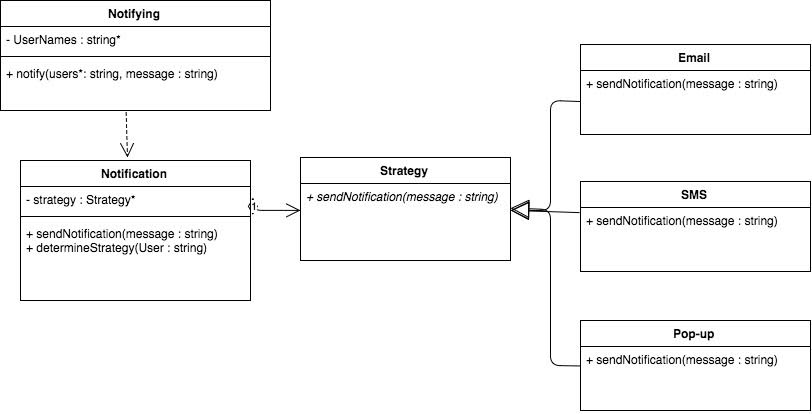
\includegraphics[width=10cm]{ClassDiagram.png}\\
\end{center}
\paragraph{Activity Diagram}
\begin{center}
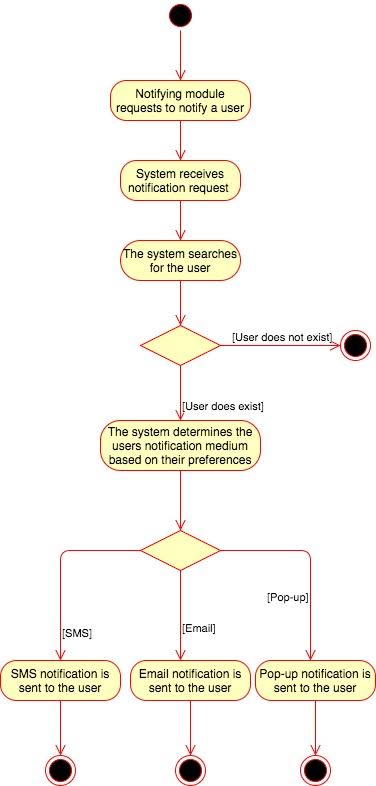
\includegraphics[height=10cm,width=5cm]{ActivityDiagram.png} 
\end{center}



\subsubsection{Technology Choices}



\subsection {Point of Interest}



\section{Technology Choices}



\section{References}

Kung, D.C. (2013) Object-oriented software engineering: An agile unified methodology. New York: McGraw Hill Higher Education.



\end{document}